\documentclass[a4paper,11pt,oneside]{article}

\usepackage [english]{babel}
\usepackage {indentfirst}
\usepackage [utf8]{inputenc}
\usepackage {fontenc}
\usepackage {amsfonts}
\usepackage {amssymb}
\usepackage [dvips] {graphicx}
\usepackage {listings}
\usepackage {latexsym}
\usepackage {alltt}
\usepackage {color}
\usepackage {fullpage}
\usepackage {amsmath}
\usepackage {geometry}
\usepackage {wrapfig}
\usepackage {setspace}
\usepackage [T1] {fontenc}
\geometry {dvips, a4paper, margin = 1 in}

\usepackage {url}
\usepackage {multicol}
\usepackage {lscape}

\usepackage {listings}
\definecolor{darkgray}{rgb}{0.95,0.95,0.95}
\lstset{language=Java}
\def\lstlistingname{Code}
\lstset{backgroundcolor=\color{darkgray}}
\lstset{basicstyle=\small,frame=leftline,captionpos=b,linewidth=\textwidth,breaklines=true,basicstyle=\ttfamily}
\setstretch{1.1}

\newcommand{\quot}[1]{`` #1 ''}

\begin{document}
% Title
\begin{titlepage}
	\title{INGI2144 Project (2011-2012) \\ RFID Loyalty Card for the LLN Sandwich Shops}
	\author{Nicolas Maître, Bernard Paulus, Arnaud Theismann}
	\date{December 12, 2011}
	\maketitle
	\thispagestyle{empty}	
	
	\vfill
	\begin{figure}[!ht]
		\centering
		
\includegraphics[scale=0.25]{Images/UCL_Logo.jpg}
		\label{fig:UCL Logo}
	\end{figure}
\end{titlepage}

\tableofcontents

\newpage
\section{Introduction}
The aim of this project was to design and implement a RFID-based system able to manage electronic loyalty cards for sandwich vendors in Louvain-La-Neuve. \\

In this document, we first present the architecture of our software and an overview of its implementation, then we give a security analysis of the whole system, along with ideas to improve it. \\


\section{Software Implementation}

\subsection{Architecture}

\begin{figure}[!ht]
	\centering
	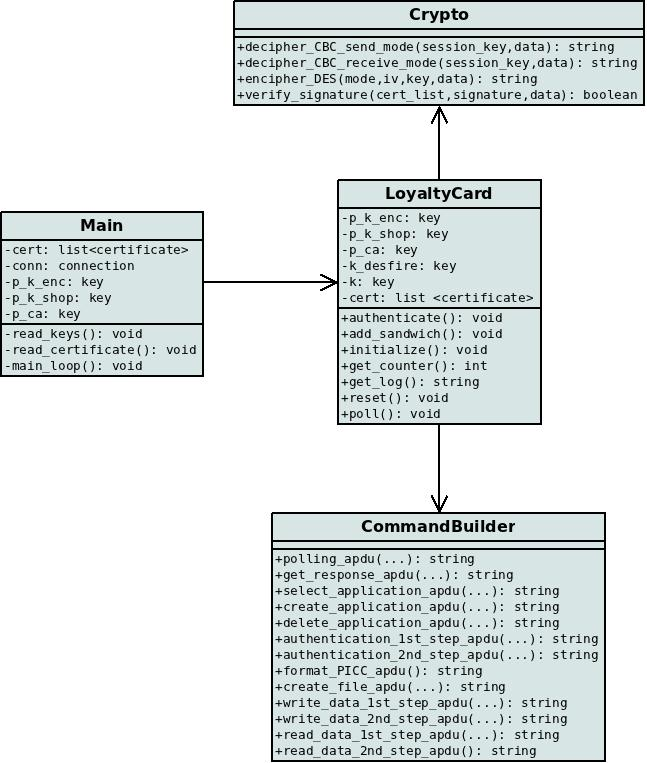
\includegraphics[scale=0.50]{Images/ClassDiagram.jpg}
	\caption{Architecture of the software}
	\label{fig:class_diagram}	
\end{figure}


As depicted on figure \ref{fig:class_diagram}, our python application is divided in 4 modules. \textbf{LoyaltyCard} class aims at representing an RFID loyalty card and offers methods to interact with. \\
\textbf{Main} is responsible to create and initialize instances of LoyaltyCard and offers to the user a command prompt to interact with the DesFire tag. Moreover, it is up to this module to load from different files the keys and certificates needed for the management of a loyalty card. \\
The \textbf{Crypto} module offers high-level cryptographic methods that are used by the \textbf{LoyaltyCard} module. These methods essentially call other methods from external crypto libraries (see next section). \\
Finally, \textbf{CommandBuilder} is a low-level module that allows to build APDUs to communicate with the tag. \\


\subsection{External tools}

In order to communicate with the RFID card, we have used \textbf{pyscard} (\url{http://pyscard.sourceforge.net}) which is a python wrapper for pcsc-lite. \\

\textbf{PyCrypto} library (\url{https://www.dlitz.net/software/pycrypto}) has been used as it provides methods for dealing with DES/3DES and RSA encryption and decryption. This python library is very interesting from a performance point-of-view since speed-critical operations like ciphers and hash functions are actually written in C. \\

In addition to this, since PyCrypto is not able to read certificates in X.509 format, we have used \textbf{M2Crypto} (\url{http://chandlerproject.org/bin/view/Projects/MeTooCrypto}) for this purpose. Retrieving public keys from certificates and verifying signatures is therefore handled thanks to this library which is in fact a wrapper for OpenSSL. \\ 

\subsection{Protection against human mistakes and bugs}

A few measures have been implemented to deal with bugs and human mistakes. First, it is impossible for the user to crash the application by performing a command when there is no RFID tag in the reader's field. Indeed, the presence of a tag is checked after every user input. If no tag is detected, a timer of 3 seconds is launched at the end of which a warning message is printed to the standard output. No further operation can be made as long as the method poll() does not return. \\

Similarly, the presence of an RFID reader is checked at application start-up. The command prompt is enabled only after the system has detected a reader. The presence of a reader is then checked every second to prevent the user from performing an operation when there is no reader. If such a case occurs, a warning message is printed to the standard output. \\ 

Finally, we ask confirmation when the user wants to reset the loyalty card to factory settings. This prevents him from erasing the whole tag memory by mistake. \\ 


\newpage
\section{Security analysis}

\subsection{Actual weaknesses of the system}

A first weakness is in the way we manage the symmetric key $K_{DESFire}$. Since this key needs to be the same for each card of a given shop, we can't generate it in a random way; the value of this key is hard-coded in the source code of the application. If an attacker were able to obtain the source code of the application, he would be able to recover this key and then erase the whole memory of a tag. \\

Similarly, the way asymmetric keys $P_{enc}$, $K_{enc}$, $P_{shop}$ and $K_{shop}$ are stored may put the system at risk. Indeed, these keys are stored in clear so as to be read by the application. Thus, each sandwich store where the application is deployed is a potential place where the keys can be stolen by an attacker.\\

Another weakness is the fact that the file containing the counter of bought sandwiches is free readable. That means that any person with a reader can determine whether a tag owner is a good client or not. This weakness may be exploited by competitors for example to target new potential clients. \\ 

An even more serious problem may be the fact that files containing the encryption E of key K and the signature S of this encryption are free readable as well. That means that an attacker would be able to obtain this data (by \textbf{skimming} the tag or \textbf{eavesdropping} the channel for example), clone it and then pretend owning a loyalty card from a legitimate sandwich vendor. Of course the attacker can't recover key K and then no shop can be abused since the logs would not be readable. But what if the attacker obtains key $P_{enc}$ by one way or another? A loyalty card would be totally clonable and no vendor would figure out. \\

The system is also vulnerable to a \textbf{replay-attack} due to the authentication mechanism. Since authentication relies on a session key, every operation requiring authentication is allowed as long as the session key is known by the prover. For a write operation, the application proves its identify by encrypting the data with the session key. That means an attacker would be able to increase its counter of sandwiches simply listening to the channel and replaying the message sent to the tag when a sandwich is bought for real. \\

Another issue is the fact that nothing prevents a seller to do malicious
tracking of its clients. Indeed, a malicious seller could identify an user by
making use of the free space left on the RFID memory. This breach is due to the
fact that new applications can be freely created because of the tag
configuration. \\

Naturally, like any other RFID-based system, our system may be vulnerable to \textbf{DOS attacks}. The first weakness described in this section is an example. An attacker may also use more generic DOS attacks such as making electronic noise to make the service unavailable. \\

\newpage
\subsection{Towards a better solution}

\subsubsection{With same technology and file/data structure}

A first improvement would be to put keys $P_{enc}$, $K_{enc}$, $P_{shop}$ and $K_{shop}$ in encrypted files protected by a password that the user needs to enter when launching the application. That would prevent an attacker from retrieving the keys and/or using the application if the executable and the keys are stolen. Similarly, $K_{DESFire}$ should be encrypted in such a file so as to make it impossible to retrieve it from the source-code. \\

Information leakage due to the free-readable counter can be easily avoided by forcing authentication with key K, just as for the logs. In this way, it is no longer possible to learn the value of this counter by skimming the tag or eavesdropping the communication channel. \\

Forcing authentication to read files containing S and E would be a solution against tag impersonation. If we want to force the authentication with key $K_{M1}$ for example, we need this key to be shared by every shop. Of course the problem is not totally solved since an attacker may obtain $K_{M1}$, but this at least provides a good defence in depth. \\


\subsubsection{With same technology only}

An interesting solution to avoid replay-attacks due to the authentication mechanism would be to force re-authentication at each write operation by changing key K. The idea would be to generate a new key K after having increased the counter and added a log. This would requires changing the key used for write operation with this new key, as well as updating E and S in files of AID 01. To do so, key settings of AID 02 should be changed to allow key change without $K_{DESFire}$. Moreover, key $K_{W1}$ should be shared by every shop, which unfortunately involves a new security flaw. \\

\section{Conclusion}

Although a graphical user interface is still missing, our implementation meets the requirements and is then ready to be put in production. We have shown that the system  still suffers from some security flaws so far, but we can assume the risk is reasonable with respect to the context of loyalty cards for sandwiches vendors. \\


\end{document}
